\documentclass[tikz]{standalone}
\usetikzlibrary{arrows.meta,math}
\usepackage{xcolor}
\begin{document}
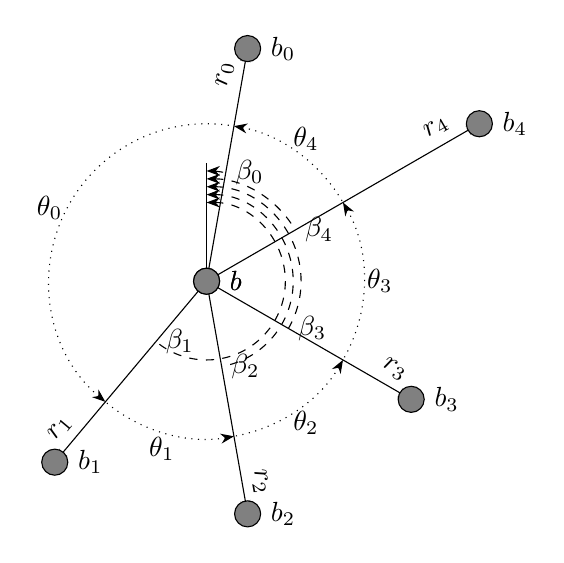
\begin{tikzpicture}[>=Stealth]
	\node[circle,fill=black!50,draw,label=right:$b$]{};
	\draw (0,0)--(up:1.5cm);
	\foreach \n/\d/\l/\a/\r in { 
			0/1.4cm/b_0/10/3cm, 
			4/1.3cm/b_4/60/4cm, 
			3/1.2cm/b_3/120/3cm,
			2/1.1cm/b_2/170/3cm,
			1/1.0cm/b_1/220/3cm 
			} {
		\draw[->] (0,0)--node[above,sloped, very near end]{$r_{\n}$} (90-\a:\r) 
					node[circle,fill=black!50,draw,label=right:$\l$]{};
		\draw[<-,dashed] (up:\d) arc[start angle=90, delta angle=-\a,
		radius=\d] node[right]{$\beta_\n$};

	};
	\foreach \n/\b/\t in { 4/10/50 , 3/60/60 , 2/120/50 , 1/170/50 , 0/220/150 } {
		\draw[dotted,<-] (90-\b:2cm) arc[start angle=90-\b, delta
		angle=-\t,radius=2cm];
		\draw (90-\b-\t/2:2.2cm) node {$\theta_\n$};
	};
	\node[circle,fill=black!50,draw,label=right:$b$]{};
\end{tikzpicture}
\end{document}

